\documentclass[border=4pt]{standalone}

\usepackage[T1]{fontenc}
\usepackage[utf8]{inputenc}
\usepackage{amsmath}
\usepackage{xcolor}
\usepackage{tikz}
\usetikzlibrary{positioning, fit, calc, arrows.meta, backgrounds}

\begin{document}
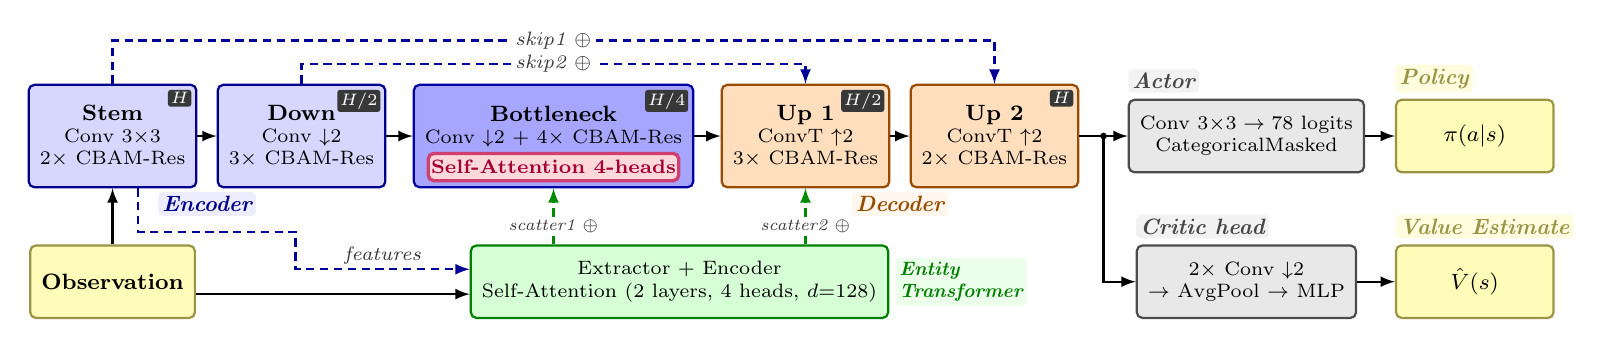
\begin{tikzpicture}[
    >=latex,
    main/.style={draw, rounded corners=2pt, minimum width=2.0cm, minimum height=1.30cm,
                 align=center, thick, inner sep=4pt, font=\scriptsize},
    enc/.style ={main, fill=blue!16,    draw=blue!55!black},
    bot/.style ={main, fill=blue!35,    draw=blue!65!black, minimum width=2.6cm},
    dec/.style ={main, fill=orange!26,  draw=orange!60!black},
    head/.style={draw, rounded corners=2pt, minimum width=2.6cm, minimum height=0.92cm,
                 align=center, thick, inner sep=4pt, font=\scriptsize,
                 fill=gray!18, draw=gray!60!black},
    flat/.style={draw, rounded corners=2pt, minimum height=0.92cm,
                 align=center, thick, inner sep=4pt, font=\scriptsize},
    ent/.style ={flat, fill=green!16,   draw=green!50!black},
    io/.style={draw, rounded corners=2pt, minimum width=2.0cm, minimum height=0.92cm,
               font=\footnotesize\bfseries, align=center, thick, fill=yellow!28,
               draw=yellow!55!black, inner sep=4pt},
    flow/.style   ={->, thick},
    skip/.style   ={->, thick, densely dashed, blue!60!black},
    scflow/.style ={->, thick, densely dashed, green!55!black},
    lbl/.style    ={font=\scriptsize\itshape, text=gray!45!black, fill=white,
                    inner sep=1.5pt},
    lblsm/.style  ={font=\fontsize{6pt}{7.2pt}\selectfont\itshape, text=gray!45!black,
                    fill=white, inner sep=1pt},
    pill/.style   ={fill=black!78, text=white, rounded corners=1pt, inner sep=1pt,
                    font=\fontsize{6pt}{7pt}\selectfont\bfseries, anchor=north east},
    grouplbl/.style={font=\footnotesize\bfseries\itshape, rounded corners=1.5pt,
                     inner sep=1.5pt, fill=white},
]

% ── Top row (y=0) — even tighter Stem-Down and Up1-Up2 ──
\node[enc]  at (1.3,  0) (ic)   {{\bfseries\footnotesize Stem}\\Conv $3{\times}3$\\$2\times$ CBAM-Res};
\node[enc]  at (3.7,  0) (down) {{\bfseries\footnotesize Down}\\Conv $\downarrow$2\\$3\times$ CBAM-Res};
\node[bot]  at (6.9,  0) (bk)   {{\bfseries\footnotesize Bottleneck}\\Conv $\downarrow$2 $+$ $4\times$ CBAM-Res\\\phantom{Self-Attention 4-heads}};
% Vivid pink/mauve Self-Attention sub-frame (slightly enlarged via inner ysep, no horizontal expansion)
\node[draw=purple!75, very thick, fill=pink!60, rounded corners=2pt,
      inner xsep=1pt, inner ysep=2.5pt, font=\scriptsize\bfseries, text=purple!85!black]
    at ($(bk.south) + (0, 0.27)$) {Self-Attention 4-heads};
\node[dec]  at (10.1, 0) (up1)  {{\bfseries\footnotesize Up 1}\\ConvT $\uparrow$2\\$3\times$ CBAM-Res};
\node[dec]  at (12.5, 0) (up2)  {{\bfseries\footnotesize Up 2}\\ConvT $\uparrow$2\\$2\times$ CBAM-Res};
\node[head] at (15.7, 0) (ac)   {Conv $3{\times}3 \to 78$ logits\\CategoricalMasked};
\node[io]   at (18.6, 0) (act)  {$\pi(a|s)$};

% Scale pills (top-right corner inside each backbone block)
\node[pill] at ([shift={(-2pt,-2pt)}]ic.north east)   {$H$};
\node[pill] at ([shift={(-2pt,-2pt)}]down.north east) {$H/2$};
\node[pill] at ([shift={(-2pt,-2pt)}]bk.north east)   {$H/4$};
\node[pill] at ([shift={(-2pt,-2pt)}]up1.north east)  {$H/2$};
\node[pill] at ([shift={(-2pt,-2pt)}]up2.north east)  {$H$};

% Encoder / Decoder labels centered below their pairs
\node[grouplbl, text=blue!55!black,   fill=blue!7]   at ($(ic.south)!0.5!(down.south) - (0, 0.20)$) {Encoder};
\node[grouplbl, text=orange!60!black, fill=orange!7] at ($(up1.south)!0.5!(up2.south) - (0, 0.20)$) {Decoder};

% Actor label at TOP-LEFT corner of actor box
\node[grouplbl, text=gray!55!black, fill=gray!10, anchor=south west]
    at ([yshift=2pt]ac.north west) {Actor};

% Policy label above π(a|s) IO box (yellow, same style as Actor)
\node[grouplbl, text=yellow!55!black, fill=yellow!12, anchor=south west]
    at ([yshift=2pt]act.north west) {Policy};

% Main flow (top row)
\foreach \a/\b in {ic/down, down/bk, bk/up1, up1/up2, up2/ac, ac/act}
    \draw[flow] (\a) -- (\b);

% Skip connections, labels at midway through dashed line
\draw[skip] (ic.north)   -- ++(0, 0.55)
    -- node[lbl, midway] {skip1 $\oplus$}
    ([yshift=0.55cm]up2.north) -- (up2.north);
\draw[skip] (down.north) -- ++(0, 0.25)
    -- node[lbl, midway] {skip2 $\oplus$}
    ([yshift=0.25cm]up1.north) -- (up1.north);

% ── Bottom row (y=-1.85, aligned to new top-row x positions) ──
\node[io]   at (1.3,  -1.85) (obs)  {Observation};
\node[ent] at (8.5, -1.85) (ent)
    {Extractor $+$ Encoder\\
     Self-Attention (2 layers, 4 heads, $d{=}128$)};
\node[head] at (15.7, -1.85) (cr)
    {$2\times$ Conv $\downarrow$2\\$\to$ AvgPool $\to$ MLP};
\node[io]   at (18.6, -1.85) (vhat) {$\hat{V}(s)$};

% Entity / Transformer label OUTSIDE ent box, to the RIGHT (vertically centered)
% 2 lines left-aligned: "Entity" and "Transformer" start at the same x
\node[font=\scriptsize\bfseries\itshape, text=green!50!black, fill=green!8,
      rounded corners=1.5pt, inner sep=1.5pt, anchor=west, align=left]
    at ([xshift=2pt]ent.east) {Entity\\Transformer};

% Critic head label at TOP-LEFT corner of critic box
\node[grouplbl, text=gray!55!black, fill=gray!10, anchor=south west]
    at ([yshift=2pt]cr.north west) {Critic head};

% Value Estimate label above V̂(s) IO box (yellow, same style as Critic head)
\node[grouplbl, text=yellow!55!black, fill=yellow!12, anchor=south west]
    at ([yshift=2pt]vhat.north west) {Value Estimate};

% Anchors on Entity Transformer left side (split into thirds for two incoming arrows)
\coordinate (entLeftUp)    at ($(ent.north west)!1/3!(ent.south west)$);  % upper third (Stem skip)
\coordinate (entLeftDown)  at ($(ent.north west)!2/3!(ent.south west)$);  % lower third (Obs)
\coordinate (obsRightDown) at ($(obs.north east)!2/3!(obs.south east)$);

% Observation → Input Conv (vertical up, BLACK)
\draw[flow] (obs.north) -- (ic.south);

% Observation → Entity Transformer (horizontal at lower third, BLACK)
\draw[flow] (obsRightDown) -- (entLeftDown);

% Entity → scatter (pure vertical, symmetric, labels lowered slightly more, smaller font)
\draw[scflow] (ent.north -| bk)  -- node[lblsm, pos=0.32] {scatter1 $\oplus$} (bk.south);
\draw[scflow] (ent.north -| up1) -- node[lblsm, pos=0.32] {scatter2 $\oplus$} (up1.south);

% Critic input branches from the Up 2 → Actor arrow (T-junction)
\coordinate (tee) at ($(up2.east)!0.5!(ac.west)$);
\draw[flow] (tee) |- (cr.west);
\fill[black] (tee) circle (1.2pt);

% Critic head → V̂(s)
\draw[flow] (cr) -- (vhat);

% Stem → Entity Transformer skip (non-additive: stem features fed to extractor)
% Z-shape from 65% of Stem width (right of Obs→Stem flow), around Encoder label, into ent's upper third
\coordinate (skStart) at ($(ic.south west)!0.65!(ic.south east)$);
\coordinate (skA) at ($(skStart) + (0, -0.55)$);
\coordinate (skB) at ($(skStart) + (2.0, -0.55)$);
\coordinate (skC) at (skB |- entLeftUp);
\draw[skip]
    (skStart) -- (skA) -- (skB) -- (skC)
    -- node[lbl, midway, above] {features} (entLeftUp);

\end{tikzpicture}
\end{document}
